%% V1.0
%% by Gabriel Garcia, gabrcg@gmail.com
%% This is a template for Udacity projects using IEEEtran.cls

%% Be Udacious!

\documentclass[10pt,journal,compsoc]{IEEEtran}

    \usepackage[pdftex]{graphicx}    
    \usepackage{cite}
    \hyphenation{op-tical net-works semi-conduc-tor}
    
    
    \begin{document}
    
    \title{Deep Learning guinea pig image classification using NVidia DIGITS and GoogLeNet}
    
    \author{\textbf{Lukasz Zmudzinski} \\ University of Warmia and Mazury in Olsztyn \\ lukasz@zmudzinski.me}
    
    %\markboth{Inference project, Robotic Nanodegree, Udacity}%
    %{}
    \IEEEtitleabstractindextext{%
    
    \begin{abstract}
    In this paper guinea pig classification using deep learning imaging methods was performed on the Nvidia DIGITS 6. Models capable of distinguishing skinny, abyssinian and crested fur types were created in the process. To increase the classification accuracy empty images (with only the background) were added to the data set. Upon evaluation, the created model recognized the animals correctly from images taken in various household backgrounds.
    \end{abstract}
    
    % Note that keywords are not normally used for peerreview papers.
    \begin{IEEEkeywords}
    classification, deep learning, animal recognition, robotics, DIGITS.
    \end{IEEEkeywords}}
    
    
    \maketitle
    \IEEEdisplaynontitleabstractindextext
    \IEEEpeerreviewmaketitle
    \section{Introduction}
    \label{sec:introduction}
    
    \IEEEPARstart{R}{obotic} systems are nowadays increasingly introduced in various animal care facilities like farms, daries and shelters \cite{agrirobo, dairyrobo}. With the growing need of automating work more methods of image classification and decision making are needed. 

    In this work, deep learning techniques were utilized to create a classification model of guinea pigs in different home environments, to explore the possibilities of bringing such systems into the world of household animals.
    
    %example for inserting image
    %\begin{figure}[thpb]
    %      \centering
    %      \caption{Robot Revolution.}
    %      \label{fig:robot1}
    %\end{figure}
    
    \subsection{Nvidia DIGITS}
    DIGITS (NVIDIA Deep Learning GPU Training System) was used in this project. It allows to rapidly train deep neural networks (DNNs) for image classification, segmentation and object detection tasks \cite{digitswww,tools}. \newline\newline
    The solution comes with pre-trained models for example:

    \begin{itemize}
        \item GoogLeNet,
        \item AlexNet,
        \item UNET and more.        
    \end{itemize}
    \noindent
    In this paper GoogLeNet was used as the model of choice.
    
    \section{Background / Formulation}
    Deep Learning is growing in popularity over the past few years. It is connected to the fact that it becomes more useful than before thanks to the amount of available training data and advances in computer hardware/software \cite{dl}. 

    Another problem with neural networks in general was vanishing gradients and unpredictable weight initialization \cite{glnp}. This becomes solved by the use of RELUs (Rectified Linear Units)\cite{relu} and more recently the GoogLeNet deep learning model\cite{dwc}.

    In neural network algorithms we can tweak several parameters, that will greately impact the final output: number of epochs, learning rate, solver type and many more.

    \begin{itemize}
        \item \textbf{Epoch} - one complete pass  of the data in the data set. The amount of epochs should be determined through tests. Small number of epochs often leads to bad predictions, while a big number leads to overfitting.
        \item \textbf{Learning rate} - describes the rate at which the network abandons old beliefs, for new ones to take their place. The value must be correct, values that are too big or too small may lead to bad predictions.
        \item \textbf{Solver type} - contains information about how the weights are updated for the network. This project used one of the most popular ones: Stochastic Gradient Descent (SGD) \cite{sgd}. 
    \end{itemize}

    Optimization algorithms help in minimizing (or maximizing on that matter) the \textit{error function}. Wide variety of pre-made optimizers are available in the DIGITS framework from the simplest gradient descents to momentum based techniques like Adagrad\cite{adagrad}.

    GoogLeNet connects various techniques known from Deep Learning like convolutions, pooling, adding softmax and more\cite{fcn}, to distinguish all the objects that are present in the image. It implements so called \textit{Inception modules}, that range from 245 filters to 1024 in top inception modules. The consequence of this is the possibility to remove fully connected layers on top completly \cite{inception}.

    \section{Data Acquisition}

    \begin{figure}[h]
        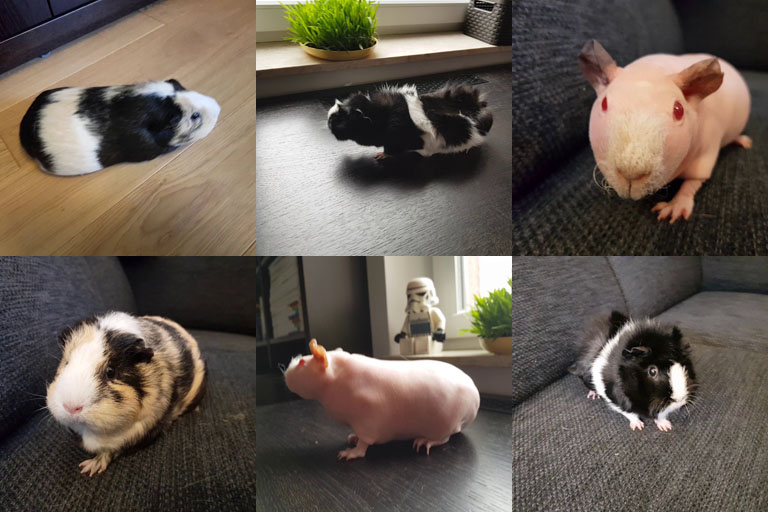
\includegraphics[width=\linewidth]{pig_dataset.png}
        \caption{Example images for crested, abyssinian and skinny guinea pigs from the provided data set.}
        \label{fig:pigs}
        \centering
    \end{figure}

    The data was collected by recording a square video of each guinea pig over a period of 30 seconds in different environments and then extracting each frame as an image. Each frame was then lowered in resolution to 256x256 px in order to fit GoogLeNet requirements. Example images can be seen in Fig. \ref{fig:pigs}.

    To ensure good accuracy of the model, each set had to cover front, side and back angles of the guinea pig body. Moreover empty images (without guinea pigs) were added of the provided backgrounds, to increase classification accuracy in distinguish items.
    \newline\newline
    Guinea pigs used in the experiment:

    \begin{itemize}
        \item Fifi (4 years, abyssinian),
        \item Rey (2 years, crested),
        \item Asajj (2 years, skinny).
    \end{itemize}

    \noindent Using the data, four labels were produced and assigned to the following neural network classes:

    \begin{itemize}
        \item \textbf{None} - when there is no guinea pig in the image,
        \item \textbf{Abyssinian}, \textbf{Crested} and \textbf{Skinny} - fur type.
    \end{itemize}

    The entire data set consisted of $1098$ images, from which 25\% were taken for validation and 10\% were excluded for testing purposes. Moreover 32 photos in different environments were taken after the training to test the model behaviour. The visual representation can be seen on Fig. \ref{fig:data}.

    \begin{figure}[h]
        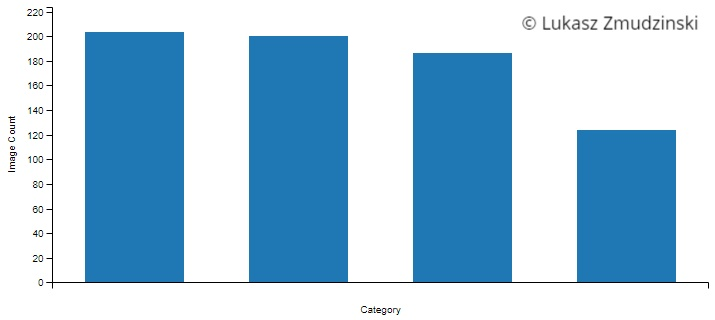
\includegraphics[width=\linewidth]{data.png}
        \caption{Data representation in the training data set. Category labels from left: crested, skinny, abyssinian, none.}
        \label{fig:data}
        \centering
    \end{figure}
    
    \section{Results}

    The final classification model was gathered from running the described image set over 15 epochs of GoogLeNet model on Nvidia DIGITS. As you can see on Fig. \ref{fig:googlenet} the accuracy after 15 epochs rose to over $90\%$, while the finall value loss was around $0.3$ with a learning rate of $0.01$. Using more epochs and a different learning was tested, but it led to overfitting of the data.

    After the model was created, a series of tests were performed to check, if the inference is correct. The first set of tests consisted of images from the previously gathered data set. The prediction was always right for provided images, with the value between 70\%-95\%. You can see an example result on Fig. \ref{fig:result_01}.

    After acquiring enough information on the predictions, tests on new images were performed (different environments, same guinea pigs) giving satisfactory results - guinea pigs were classified correctly on each provided picture containing the animal. Example result on Fig. \ref{fig:result_02}.

    One failed prediction was encountered, when a picture of a background with a cat was used. The cat was badly classified as an abyssinian guinea pig.

    \begin{figure}[h]
        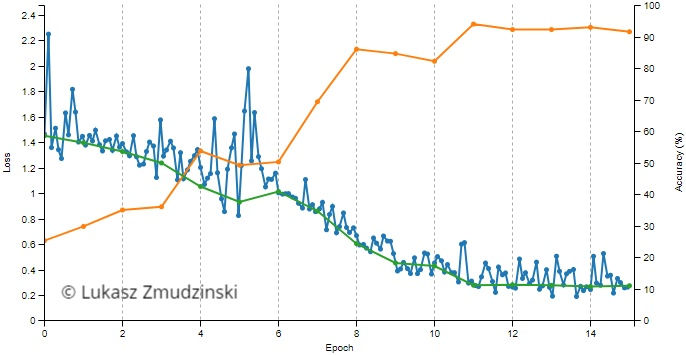
\includegraphics[width=\linewidth]{googlenet.png}
        \caption{Graph showing the value accuracy (orange), test data loss (blue) and value loss (green) after running the GoogLeNet model.}
        \label{fig:googlenet}
        \centering
    \end{figure}

    \begin{figure}[h]
        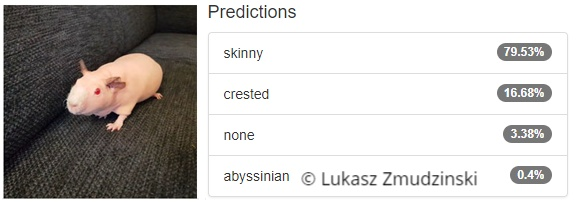
\includegraphics[width=\linewidth]{result_01.png}
        \caption{Example correct prediction results (79.53\%) using previously captured images in selected environments using GoogLeNet.}
        \label{fig:result_01}
        \centering
    \end{figure}

    \begin{figure}[h!]
        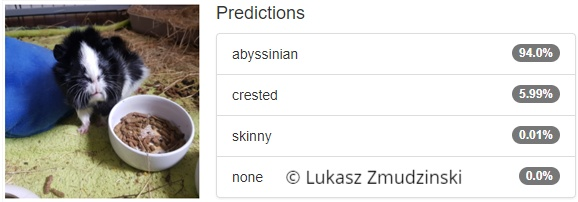
\includegraphics[width=\linewidth]{result_02.png}
        \caption{Example correct prediction results (94.0\%) using post-model captured images in animal cage environment using GoogLeNet.}
        \label{fig:result_02}
        \centering
    \end{figure}
    
    \section{Discussion}
    Modern robotics highly depend on sensor readings of the surrounding environment. They often use camera input as one of the parameters to perceive the world. Due to that, imaging methods for decision-making were introduced.

    Related works about animal classification were published in regard of wild animal monitoring \cite{wild, trap2} and classifying different animals from their own data sets\cite{trap}. The authors follow a similar pattern when using deep neural networks, but none of them concern household animals. Both projects face different problems from those, that could be encountered in a safe, indoor environment. Hence, different data acquisition techniques had to be used. 

    In this paper Deep Learning was implemented for guinea pig classification in order to explore the possibilities of introducing household animal care using robotics and automation, while keeping them safe.

    The provided GoogLeNet model from NVidia DIGITS has proven successful in identifying the guinea pigs in different environments, even when taking images that weren't originally added to the data set. Some errors were observed (false-positives) when no guinea pigs were present in the tested image. The model will behave poorly when other animals are present in the pictures, since the classification was based purely on guinea pigs.

    Increasing the accuracy of the model, can greately improve the robot-animal interactions, allowing to tailor behaviours to specific beings. This could be achieved by using modifying the learning rate, using more images, creating more labels or finally using a different optimizer or pre-built model. There are many possible variables to take into consideration, when building a model for a defined task.

    The guinea pig classification model after building with GoogLeNet, was able to provide results almost instantly. This is important, if used for robotics, because while waiting for an action, the environment can change quite drasticly. Moreover, such model are built to be deployed on an autonomous platform (Raspberry, Jetson TX2 or any other), so the memory usage will be limited, increasing the inference calculation time.
    
    \section{Conclusion / Future work}
    The created model proves that guinea pig fur recognition for robotic systems is possible. The project gave good results - the created model recognized the animals correctly from images taken in various household backgrounds. The prediction was acquired fast making the inference time low. This is especially important for robotic systems that deal with live animals, because the reaction times need to be rapid. 

    Future work might include robotic systems that monitor the state of specific animals, adjust food distribution depending on image readings or alert when the guinea pig suffers from any kind of illness.

    Moreover, different types of models can be employed to see, which one fits the needs the most. The project shouldn't be limited to GoogLeNet.
    
   \bibliography{bib}
   \bibliographystyle{ieeetr}

   \newpage
    \section{Udacity provided data}

    All the necessary project requirements for the supplied data were placed in this section. My plan is to publish the paper as an actual scientific article, so need to separate the Udacity challenge from the actual guinea pig project.\newline

    \noindent The following steps were taken to create the Conveyor Belt model:

    \begin{enumerate}
        \item The DIGITS platform was started,
        \item {
            Provided image data set was downloaded to "Conveyor Belt" image classification set. The data settings were:
            \begin{itemize}
                \item Image dimensions: 256x256
                \item Image type: Color
                \item Resize Transformation: Squash
                \item DB Backend: lmdb
                \item Image encoding: png
                \item DB Compression: none
            \end{itemize}
            The whole dataset took: 675 mb.
        }
        \item {
            A new Image Classification Model was created with the following settings:
            \begin{itemize}
                \item Training epochs: 15,
                \item Solver type: Adagrad,
                \item Base Learning Rate: 0.01,
                \item Network used: GoogLeNet standard network.
            \end{itemize}
            After some time, I broke the model creation, because after 6 epochs, no changes were seen on the graph.
        }
        \item {
            The \textbf{evaluate} was run on the model, providing the results as seen on Fig. \ref{fig:udacity}:
            \begin{itemize}
                \item Average time: 4.95ms
                \item Model accuracy: 75.41\%
            \end{itemize}
        }
    \end{enumerate}

    \begin{figure}[h!]
        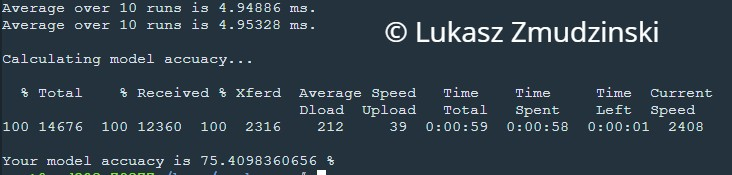
\includegraphics[width=\linewidth]{udacity.png}
        \caption{The results of the evaluate methods for Udacity data set.}
        \label{fig:udacity}
        \centering
    \end{figure}
\newpage
    \subsection{Conclusion}
    The Conveyor Belt project ended up quite similar to the Guinea Pig that was created earlier. The inference time achieved was really good - around 5ms. That means that the robot, will get the data about the object almost instantly. The accuracy was just over 75\%, which makes the passing rate, although could be improved, by playing with the model parameters.
    \end{document}